

\documentclass[sigconf]{acmart}

%DON'T CHANGE THIS FILE
%This file sets several properties for the ACM template.
%It is not necessary to change this file.


% Copyright
\setcopyright{none}

% DOI
\acmDOI{}

% ISBN
\acmISBN{}

%Conference
\acmConference[Praktikum Elektrische Maschinen]{}
\acmBooktitle{}
\copyrightyear{2021}

\newcommand{\supervisors}[1]{\thanks{Betreut von #1}}




%In the preamble file you can include packages and define macros.
\usepackage{xspace}
\usepackage[ngerman,english]{babel}
\usepackage{graphicx,lipsum}
\usepackage[europeanvoltages,
europeancurrents,
europeanresistors,
americaninductors,
smartlabels,siunitx,straightvoltages]{circuitikz}
\usepackage{float}
%Here we define a marco: The \xspace ensures correct spacing, i.e. insert space before next word, but not before period or comma.
\newcommand{\paxos}{\textsc{Paxos}\xspace}

%These packages are needed for the plot in Figure 1. 
\usepackage{tikz}
\usepackage{pgfplots}
\pgfplotsset{compat=newest}


\begin{document}
%TODO: Title 
\title{Drehstromtransformator}
%TODO: Subitle 
\subtitle{Elektrische Energieversorgung}

%TODO authors 
\author{Ahmed Habib, Lukas Nöller}

%TODO affiliation 
\affiliation{HTW Dresden}
%\email{email@somedonain}

%TODO: change language according to class 
\selectlanguage{ngerman} 

%TODO: supervisors
\supervisors{Prof. Dr.-Ing. Gerd Valtin }

\maketitle


\section{Enführung}
%\label{sec:introduction}
\lipsum

\begin{figure}
    \begin{small}
        \begin{center}
            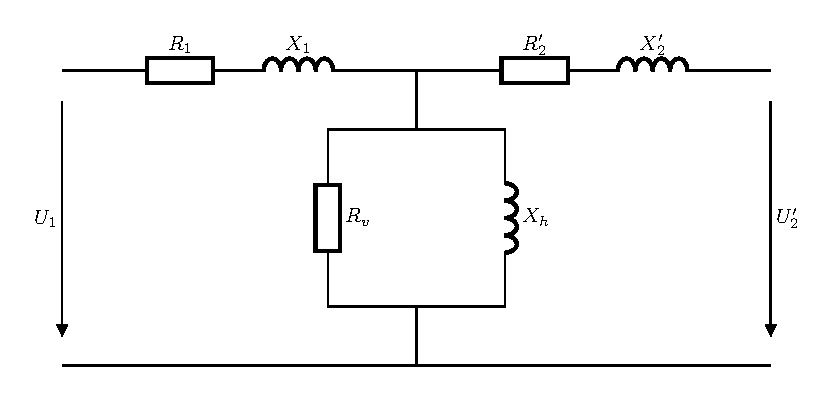
\includegraphics[width=0.95\columnwidth]{fig/eq.pdf}
        \end{center}
        \caption{EQUIV CIRC}
        \label{fig:eq}
    \end{small}
\end{figure}


\section{Experimental Evaluation}
\label{sec:evaluation}
Here you evaluate your work using experiments. You start
again with a very short summary of the section. The typical
structure follows.

\subsection{Experimental setup}
Specify the context and setup of your experiments. This includes e.g.~what hardware (VMs) you are running on, what operating system these machines are running, how they are connected, ...

Also explain how you generate load for your system and what parameters you used here. The general idea is to include enough information for others to reproduce your experiments. To that end, you should provide a detailed set of instructions for repeating your experiments. These instructions should not be included in the report, but should be provided as part of the source code repository on GitHub, typically as the \texttt{README.md} file, or as Shell scripts or Ansible scripts.

If your experiments give strange or unexpected results, analyze, profile and debug your code. \textbf{Do not simply re-run experiments until they give the expected results.}

Finally, running experiments is very time consuming and you may need to go through multiple rounds of experiment, debugging and optimization. \textbf{Do not delay running experiments until the end of your project period.} 

\subsection{Results}
The results of your experiments. Compare different variants of your design (e.g.~with and without optimizations) or compare performance to other designs or systems. Plots should show the average over multiple runs (at least 10 as a rule of thumb), including error bars, percentiles or min/max values.

Discuss the plot and extract the overall performance. Do not repeat all numbers in the text, but mention relevant differences in numbers, e.g.~our optimization improves throughput by 26\%.
Discuss how the results validate or contradict your assumptions.

Perform experiments to evaluate your system under operating normal conditions, when experiencing failures or attacks, or with different workloads.

Figure~\ref{fig:graph} shows a graph generated with \texttt{pgfplots} from 
experiment data.
\begin{figure}
\begin{tikzpicture}
\begin{axis}[
    /pgf/number format/.cd,
        use comma,
        1000 sep={},
        xlabel=$U_{1L}$,
        ylabel=$U_{2L}$,
    %legend entries={baseline, optimized},
]
%The mockup experiment data is stored in a csv file, and imported here.
\addplot table [x=U_1L, y=U_2L, col sep=comma] {data/leerlauf.csv};
%\addplot table [x=U_1L, y=ue, col sep=comma] {data/leerlauf.csv};
\end{axis}
\end{tikzpicture}
\caption{A graph showing latency and throughput of a baseline and optimized implementation. The axes show latency in milliseconds, and throughput in thousand operations per second. Data is made up.}
\label{fig:graph}
\end{figure}

\begin{figure}
    \begin{tikzpicture}
    \begin{axis}[
        /pgf/number format/.cd,
        use comma,
        1000 sep={},
        xlabel=$U_{1L}$,
        ylabel=Ü,
        %legend entries={baseline, optimized},
    ]
    %The mockup experiment data is stored in a csv file, and imported here.
    %\addplot table [x=U_1L, y=U_2L, col sep=comma] {data/leerlauf.csv};
    \addplot table [x=U_1L, y=ue, col sep=comma] {data/leerlauf.csv};
    \end{axis}
    \end{tikzpicture}
    \caption{A graph showing latency and throughput of a baseline and optimized implementation. The axes show latency in milliseconds, and throughput in thousand operations per second. Data is made up.}
    \label{fig:graph}
    \end{figure}

    \begin{figure}
        \begin{tikzpicture}
        \begin{axis}[
            /pgf/number format/.cd,
            use comma,
            1000 sep={},
            xlabel=$I_{2kL}$ (A),
            ylabel={$ U_{1kL} (\mathrm{V}), \quad I_{2kL}$ (A)},
            legend entries={$U_{1kL}$, $I_{2kL}$},
            legend pos=north west,
        ]
        %The mockup experiment data is stored in a csv file, and imported here.
        \addplot table [x=I_2kl, y=U_1kl, col sep=comma] {data/kurzschlussversuch.csv};
        \addplot table [x=I_2kl, y=I_2kl, col sep=comma] {data/kurzschlussversuch.csv};
        \end{axis}
        \end{tikzpicture}
        \caption{A graph showing latency and throughput of a baseline and optimized implementation. The axes show latency in milliseconds, and throughput in thousand operations per second. Data is made up.}
        \label{fig:graph}
        \end{figure}
        
    


\section{Conclusion}
\label {sec:conclusion}
Here you need to summarize what you did and why this is
important. Do not take the abstract and put it in the past
tense. Remember, now the reader has (hopefully) read the
paper, so it is a very different situation from the abstract.
Try to highlight important results and say the things you really
want to get across such as high-level statements (e.g.,
we believe that .... is the right approach to .... Even though
we only considered LAN, the .... technique should be applicable
....) You can also formulate next steps if you want.
Be brief.


\end{document}
